\chapter{Музыкальные композиции}
\label{ch:musical-composition}
Глава посвящена исследованию музыкальных композиций. 
С помощью SPARQL-запросов, вычисляемых на объектах типа <<музыкальная композиция>> в~Викиданных, 
получены списки музыкальных композиций, список наиболее плодовитых композиторов, 
найдены популярные музыкальные жанры. 
Получен список музыкальных произведений в Викиданных, 
для которых будет законно зарузить их аудиозапись на Викисклад, поскольку истек срок копирайта.

\section{Число <<Музыкальных композиций>> и жанры}

\marginnote{Используемые в запросах объекты: <<\wdqName {музыкальное произведение/композиция} {105543609}>>;
используемое свойство: <<\wdProperty{31}{экземпляр}>>.}

Построим список всех музыкальных композиций с помощью запроса~\ref{lst:musical_composition}.

\begin{lstlisting}[ 
    language=SPARQL,
    caption={\href{https://w.wiki/9TcJ}{Список всех  музыкальных композиций}\protect\footnotemark},
    label=lst:musical_composition,
    texcl,
    numbers=none
    ]
# List of all musical compositions
SELECT ?composition ?compositionLabel
WHERE {
  ?composition wdt:P31 wd:Q105543609. # instance of musical work/composition
  SERVICE wikibase:label { bd:serviceParam wikibase:language "ru,en" }
}
\end{lstlisting}%
\footnotetext{Получено: \num{5495} записей на 2017 год и \num{150,5} тыс. записей на~2023 год. 
        Ссылка на~SPARQL-запрос: \href{https://w.wiki/9TcJ}{https://w.wiki/9TcJ}.}

Наиболее полными и проработанными примерами музыкальных композиций на Викиданных являются: <<\wdqName{Волшебная флейта}{5064}>>, <<\wdqName{К Элизе}{11980}>>, <<\wdqName{Реквием}{207875}>>, <<\wdqName{Маленькая ночная серенада}{12025}>>, <<\wdqName{Соната си синор}{63681379}>>.

В 2022 году по запросу~\ref{lst:musical_composition} найдено \num{106,7} тыс. музыкальных композиций, 
а~в~2023~--- \num{150,5} тыс., вместо \num{5,5} тыс. в~2017 году. 
Увеличение числа композиций связано с тем, что эти объекты Викиданных являются теперь не экземплярами объекта «музыкальное произведение», а экземплярами различных подклассов «музыкальное произведение». При поиске подклассов объекта «музыкальное произведение» можно найти такие жанры: <<\wdqName{песня}{7366}>>, <<\wdqName{духовная песня}{856713}>>, <<\wdqName{гимн}{484692}>>. Более подробно анализ музыкальных жанров будет представлен в разделе <<Количество музыкальных произведений по~жанрам>> на стр. 96.

\todoVlad{\TODO Владимир, так не годится писать плейнтекстом: <<на стр. 96>>, 
поскольку, например, в этом PDF-файле всего 49 страниц. 
Используйте команду pageref с аргументом label, 
который задаётся в~начале того раздела, на который Вы хотите сослаться. 
И между предлогом и словом нужен неразрывный пробел. 
Тогда получится, например так:} 
\begin{verbatim}
на~с.~\pageref{ch:BucketsAndBalls}. 
\end{verbatim}
\todoVladWithoutCounter{Здесь в начале метки ``ch:BucketsAndBalls'' стоит ``ch''~--- 
это сокращение от chapter (глава), 
чтобы не путать с другими метками (таблицами, рисунками).}

\todoVlad{Добавьте здесь текстовое описание к рис.~\ref{fig:hier-music}.  
\newline 
\newline
P.S. Владимир, не удаляйте эти задания из текста.}

\answerVlad{Владимир, а в таких блоках текста, когда задание выполнено, 
то пишите, пожалуйста, <<Готово>> или <<Сделано>>. 
Либо напишите пояснение, что не сделано и объясните~--- почему.}


\begin{marginfigure}[0\baselineskip]
	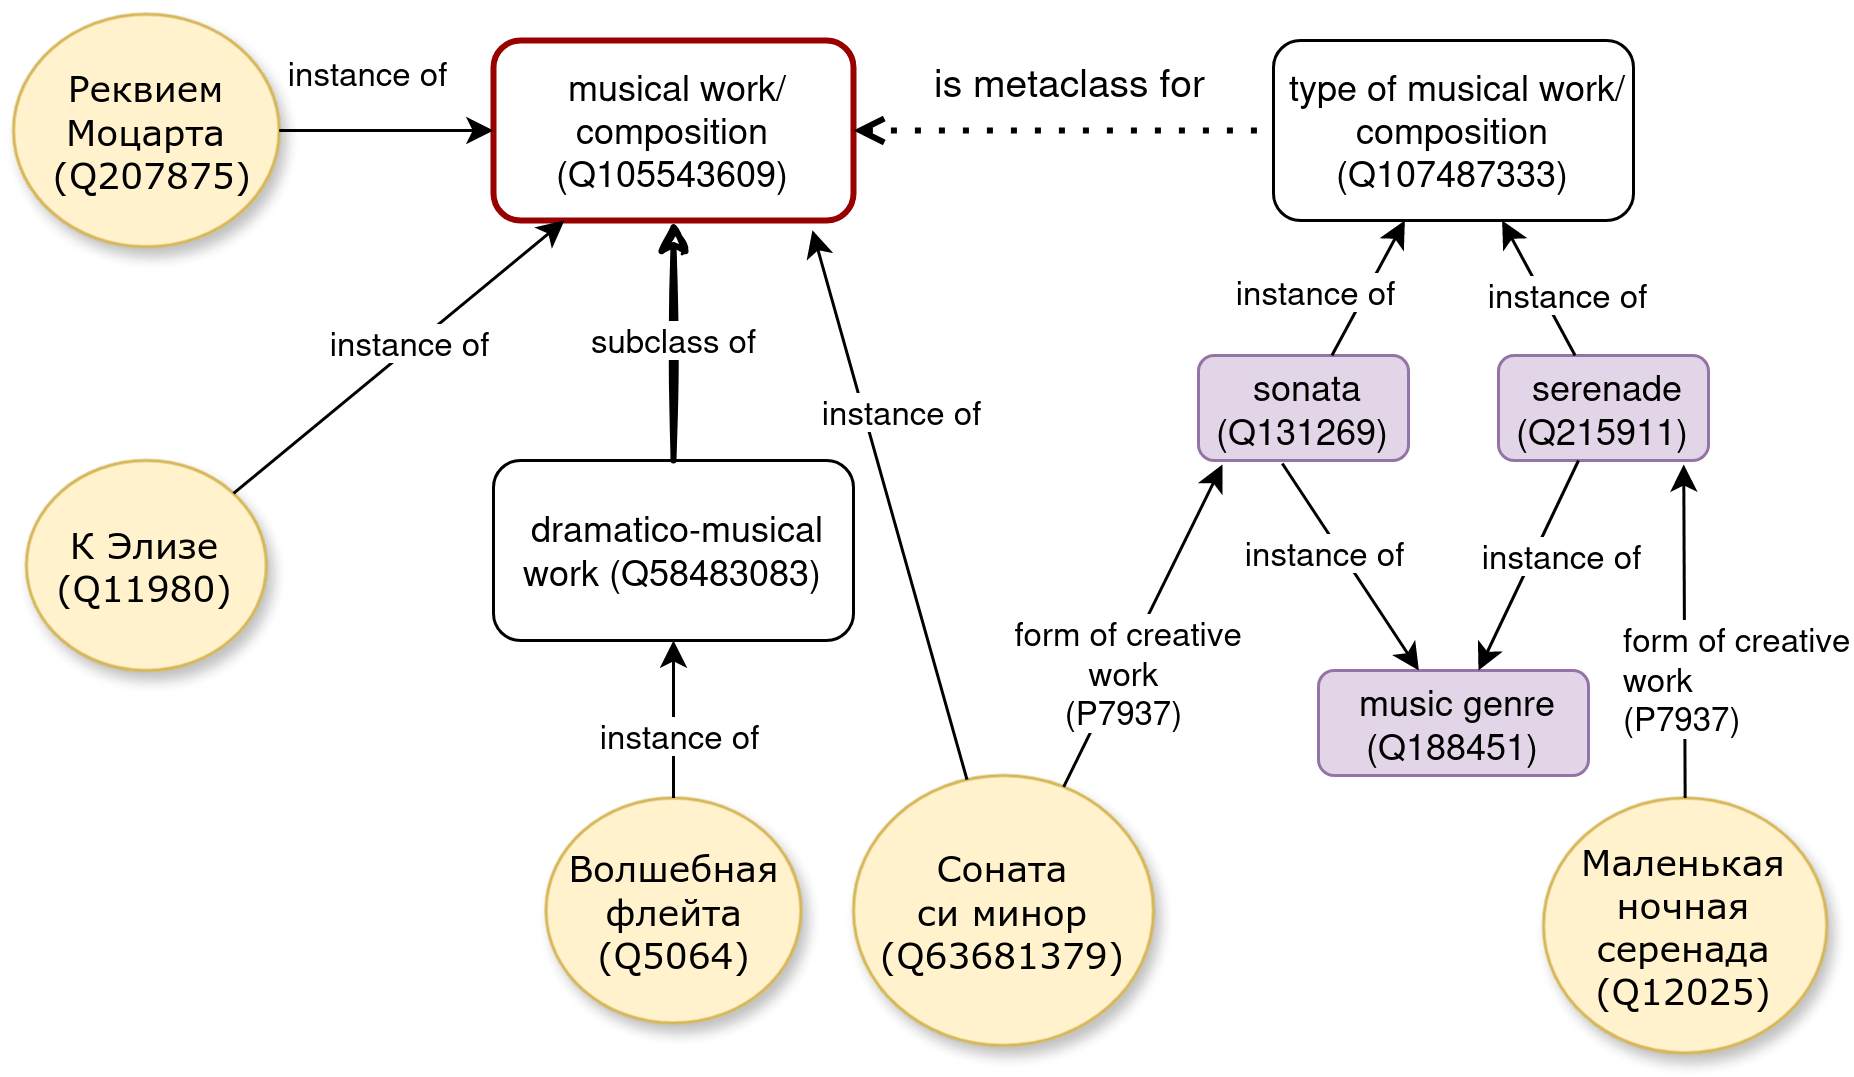
\includegraphics[width=1\textwidth]{./chapter/musical_composition/hierarchy_of_music_classes_WD_2023.png}
	\caption[Иерархия музыкальных классов]{Фрагмент иерархии музыкальных классов в Викиданных, 2023 год}%
	\label{fig:hier-music}%
\end{marginfigure}
Найдём количество музыкальных композиций в каждом жанре с помощью запроса~\ref{lst:music _in_each_subclass}.

\begin{lstlisting}[ 
    language=SPARQL,
    caption={\href{https://w.wiki/8PzR}
                  {Количество музыкальных композиций в каждом подклассе}\protect\footnotemark},
    label=lst:music _in_each_subclass,
    texcl
    ]
# Count of pieces of music in each subclass
SELECT ?type (COUNT(?typeInstance) AS ?count) ?typeLabel WHERE {
  ?type wdt:P279* wd:Q105543609.    # subclass of musical composition
  ?typeInstance wdt:P31 ?type.      # instance of this subclass 
  SERVICE wikibase:label { bd:serviceParam wikibase:language "ru, en" }
}
GROUP BY ?type ?typeLabel
ORDER BY DESC (?count)
\end{lstlisting}%
\footnotetext{Получено: \num{161} подкласс музыкальных композиций на 2022 год. Ссылка на SPARQL-запрос: \href{https://w.wiki/8PzR}{https://w.wiki/8PzR}.}


\todoVlad{После предыдущего запроса~\ref{lst:music _in_each_subclass} 
обратите внимание читателя, 
что в этом запросе используется только левая часть рис.~\ref{fig:hier-music}, 
а именно:  ``musical work/composition (Q105543609)''. 
Поэтому в подклассах нет ни сонаты, ни серенады. 
Владимир, предлагаю Вам добавить в запрос объект ``type of musical work/composition (Q107487333)'' 
и искать в том числе и по подклассам этого объекта, то есть результатов должно стать больше. 
В результатах должны появиться жанры: соната и серенада~--- проверьте это.}

\todoVlad{Общее пожелание. Добавьте к запросам, которые возвращают числа~--- данные за 2024 год, 
при этом оставляйте данные (число результатов) за предыдущие годы.}

Теперь подсчитаем общее суммарное число музыкальных произведений с учётом музыкальных композиций в подклассах. Для этого добавим в~запрос~\ref{lst:music _in_each_subclass} команду \lstinline|SUM()| в~строку~2 и удалим лишние строки, чтобы получить запрос~\ref{lst:The_total_number_of_musical_works_for_all_subclasses}.


\begin{lstlisting}[ 
    language=SPARQL,
    caption={\href{https://w.wiki/9Tc3}
                  {Суммарное число музыкальных произведений 
                   с~учётом музыкальных композиций в~подклассах}\protect\footnotemark},
    label=lst:The_total_number_of_musical_works_for_all_subclasses,
    texcl,  
    xleftmargin=18pt
    ]
# The total number of musical works for all subclasses 
SELECT (SUM(?count) AS ?sum) WHERE{
  SELECT (COUNT(?music) AS ?count) WHERE {
                         # subclass of musical work/composition
                   ?type wdt:P279* wd:Q105543609.
    ?music wdt:P31 ?type
  }        # instance of this subclass
}
\end{lstlisting}%
\footnotetext{Получено: 145~тыс. музыкальных произведений на 2022 год, 
    164~тыс. на 2023 год и 170~тыс. на 2024 год. 
    Ссылка на~SPARQL-запрос: \href{https://w.wiki/9Tc3}
                                  {https://w.wiki/9Tc3}.}

Можно записать этот код ещё короче. 
Переменная \lstinline|?type| нам не нужна, 
поэтому заменим её на \emph{безымянную переменную}, \index{SPARQL![]!безымянная переменная}
а~строки 5 и 6 поменяем местами, 
получаем запрос~\ref{lst:The_total_number_of_musical_works_for_all_subclasses_up}.

\begin{lstlisting}[ 
    language=SPARQL,
    caption={\href{https://w.wiki/9Td7}
                  {Суммарное число музыкальных произведений с~учётом музыкальных композиций 
                  в~подклассах (безымянная переменная)}\protect\footnotemark},
    label=lst:The_total_number_of_musical_works_for_all_subclasses_up,
    texcl,
    numbers=none
    ]
# Total number of musical works for all subclasses
SELECT (SUM(?count) AS ?sum) WHERE{
  SELECT (COUNT(?music) AS ?count) WHERE {
    ?music wdt:P31   # instance of
          [wdt:P279* wd:Q105543609].
  }        # subclass of musical work/composition
}
\end{lstlisting}%
\footnotetext{Идентичный запрос предыдущем, то же число результатов. Ссылка на~SPARQL-запрос: \href{https://w.wiki/9Td7}{https://w.wiki/9Td7}.}

По сравнению с 2017 годом, когда было получено \num{5494} записи, число записей увеличилось в десятки раз. Это связано с тем, что за 5 лет было добавлено множество новых музыкальных произведений, а также старых, которые не были учтены ранее.
Напишем скрипт~\ref{lst:Musical_comp_2018--2023} и посмотрим сколько новых и старых (то есть созданных до 2018 года) музыкальных произведений было добавлено в~Викиданные за~период с~2018 года по~2023 год.

\todoVlad{Раз мы добрались до этого года в нашей работе, то замените, пожалуйста, 
2023 на 2024 и обновите здесь и далее результаты. 
Выше тогда напишите <<за 6 лет>>, а не за пять лет.}

\begin{lstlisting}[ 
    language=SPARQL,
    caption={\href{https://w.wiki/9RYq}{ Количество музыкальных композиций в период 2018--2023 годы}\protect\footnotemark},
    label=lst:Musical_comp_2018--2023,
    xleftmargin=18pt,
    numbers=left,
    ]
# The total number of musical works for all subclasses 
SELECT (SUM(?count) AS ?sum) WHERE{
  SELECT (COUNT(?music) AS ?count) WHERE{
    ?music wdt:P31 wd:Q105543609;  # subclass of musical composition
           wdt:P577 ?publication.  # has a publication date
    BIND(YEAR(?publication) AS ?year)
    FILTER(?publication > "2018-01-01T00:00:00Z"^^xsd:dateTime)
  }
}
\end{lstlisting}%
\footnotetext{Получено: \num{3234} музыкальных произведений за 2018--2023 годы. Ссылка на SPARQ-запрос: \href{https://w.wiki/9RYq}{https://w.wiki/9RYq}.}

\todoVlad{Владимир, я вернул в запрос~\ref{lst:Musical_comp_2018--2023} нумерацию строк. 
Владимир, я не понял, почему Вы удалили нумерацию. 
Можете посмотреть сканы в ТГ от 13 декабря, которые я Вам присылал, насчитал там 6 скриптов с нумерацией. 
Прошу вернуть нумерацию строк в те скрипты, на номера строк которых есть отсылки из текста.}

\todoVlad{Владимир, в запросе~\ref{lst:Musical_comp_2018--2023} 
есть такая строка \lstinline|BIND(YEAR(?publication) AS ?year)|. 
Забавно, но переменная ?year, задаваемая в этой строке, в скрипте не используется. 
Перепишите строку 7 с командой FILTER, чтобы использовалась переменная ?year (вариант без FILTER). 
В тексте после запроса напишите, что\newline 
(1: вариант с FILTER) можно использовать такую тяжёлую конструкцию 
\lstinline|FILTER(?publication > "2018-01-01T00:00:00Z"^^xsd:dateTime)|, 
но зато не нужна строка 6 с командой \lstinline|BIND|,\newline 
либо\newline
(2: вариант без FILTER) более читаемый код с командой \lstinline|BIND| 
и переменной \lstinline|?year|. \newline
В листинге будет только вариант (2), в тексте~--- оба. 
В тексте пишите строчки кода или команды SPARQL с помощью конструкции lstinline.}



Запрос~\ref{lst:The_total_number_of_musical_works_for_all_subclasses_up} 
возвращает 164 тыс. музыкальных произведений, которые могут иметь или не~иметь дату публикации. 
В~запросе~\ref{lst:Musical_comp_2018--2023} в~строке~5 
мы требуем обязательного наличия свойства <<\wdProperty{577}{дата публикации}>> у музыкального произведения.
Таких произведений с заполненной датой публикации 
(и выключенной, 
 то есть закомментированной строкой~7 в~запросе~\ref{lst:Musical_comp_2018--2023}) найдено 51 тыс., 
то есть примерно в~3~раза меньше. 
Если фильтрация в~строка~7 запроса~\ref{lst:Musical_comp_2018--2023} включена, 
то получаем 3.2 тыс. новых произведений, опубликованных не~ранее 2018 года. 
Получается, что таких достоверно <<новых>> музыкальных произведений 
около 2\,\% (3.2 тыс.) от всех музыкальных произведений в Викиданных (164 тыс.).






\section{Количество музыкальных произведений по годам}

Подсчитаем количество музыкальных произведений 
со второй половины XIX века до настоящего времени 
с~помощью запроса~\ref{lst:The_number_of_musical_compositions_for_every_10_years}. 
Этот запрос строит рис.~\ref{fig:diagram_10_years}, где 
указано число созданных произведений по десятилетиям. 


\index{SPARQL!wikibase!isSomeValue}
\begin{lstlisting}[ 
    language=SPARQL,
    caption={\href{https://w.wiki/7wHy}
                  {Количество музыкальных произведений, создаваемых каждое десятилетие}\protect\footnotemark},
    label=lst:The_number_of_musical_compositions_for_every_10_years,
    texcl,
    numbers=none
    ]
# The number of musical compositions for every 10 years
#defaultView:BarChart
SELECT (STR(?date) AS ?date_str) (COUNT(?composition) AS ?count) WHERE {
  ?composition wdt:P31 wd:Q105543609;     # instance of compostion
    wdt:P86 ?composer;                    # composition has a composer
    wdt:P577 ?publication.                # composition has a publication date
  BIND(YEAR(?publication) AS ?year)
  BIND((FLOOR(?year / 10 )) * 10  AS ?date)
  FILTER(?publication > "1850-01-01T00:00:00Z"^^xsd:dateTime)
  FILTER(?publication < "2030-01-01T00:00:00Z"^^xsd:dateTime) 
  FILTER (!wikibase:isSomeValue(?publication)) # field "date" must be filled
}
GROUP BY ?date
ORDER BY (?date)
\end{lstlisting}%
\footnotetext{Ссылка на SPARQL-запрос: \href{https://w.wiki/7wHy}{https://w.wiki/7wHy}.}

\begin{marginfigure}[-5\baselineskip]
    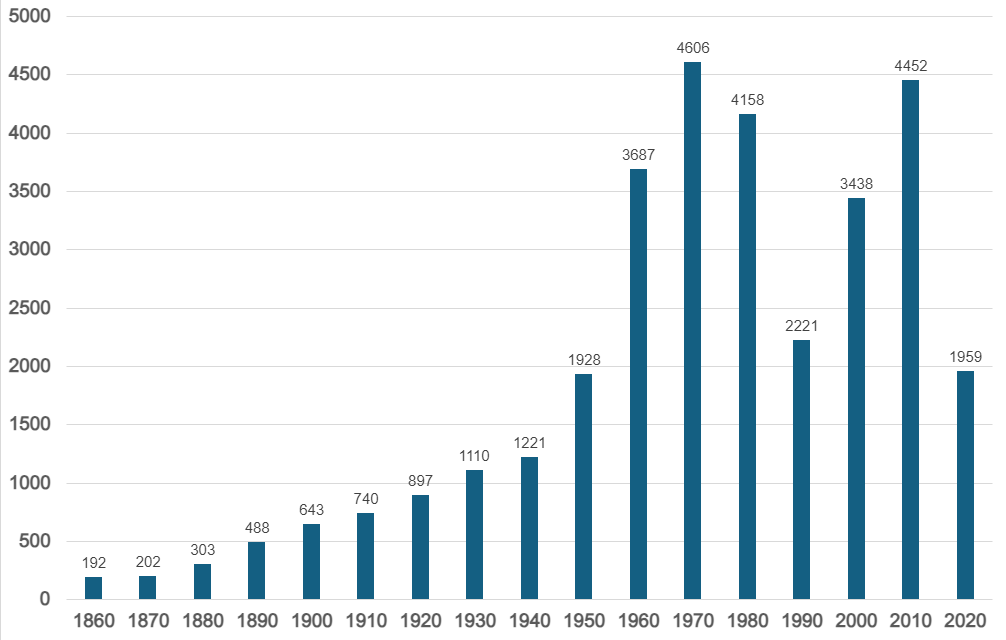
\includegraphics[width=1\textwidth]{./chapter/musical_composition/BarChart_of_The_number_of_music_compositions_for_every_10_years.svg.png}a
    \vspace{-7pt}
	\caption{Гистограмма количества музыкальных произведений, 
             создаваемых каждое десятилетие со второй половины XIX века до настоящего времени}%
	\label{fig:diagram_10_years}%
\end{marginfigure}
%
Рис.~\ref{fig:diagram_10_years} показывает, что до 1890 года (1850--1890 годы) 
количество написанных музыкальных произведений невелико. 
После 1890 года (1890--1970 годы) начинается резкий подъём числа новых произведений 
и продолжается до нашего времени. 
Такое увеличение музыкальных произведений можно объяснить тем, 
что со временем появляются новые жанры и новые устройства для записи. 
На гистограмме (рис.~\ref{fig:diagram_10_years}) видим два пика: 1960--1980-е, 2000-е и 2010-е.

\todoVlad{Владимир, у скриншота (рис.~\ref{fig:diagram_10_years}) низкое качество 
(то есть текст размытый при увеличении), 
переснимите, пожалуйста, с большим разрешением. 
На рис.~\ref{fig:diagram_10_years} нужно сделать крупные подписи по обеим осям (название оси и числа). 
Можете доработать в графическом редакторе. 
Не забудьте новые версии рисунков загружать на Викисклад 
(можно поверх старых, чтобы не писать заново описание файла) 
и новые рисунки включайте в свою страницу в Викиверситете, то есть сюда: 
\textit{Программирование Викиданных/Музыкальные композиции}.}






\newpage
\section{Количество музыкальных произведений по жанрам}

Найдём, в каких жанрах были написаны музыкальные произведения 
в пиках графика (рис.~\ref{fig:diagram_10_years}) 
и~изобразим жанры на~круговой диаграмме (рис.~\ref{fig:Genre_Chart_1960_—_1980}), 
полученной по запросу~\ref{lst:count_of_pieces_of_music_in_each_subclass}. 
Рассмотрим первый пик, приходящийся на~1960--1980-е годы, назовём этот пик <<Первая волна>>.

\begin{marginfigure}[0\baselineskip]
	\includegraphics[width=1\textwidth]{./chapter/musical_composition/Genre_Chart_1960_—_1980.png}
	\caption[Круговая диаграмма музыкальных жанров за 1960--1980 годы во всем мире]{Круговая диаграмма музыкальных жанров за 1960--1980 годы во всем мире. Ссылка на SPARQL-запрос: \href{https://w.wiki/6Vx5}{https://w.wiki/6Vx5}.}%
	\label{fig:Genre_Chart_1960_—_1980}%
\end{marginfigure}

\begin{lstlisting}[ language=SPARQL,
                    caption={\href{https://w.wiki/6Vx5}{ Количество музыкальных произведений в каждом жанре}\protect\footnotemark},
                    label=lst:count_of_pieces_of_music_in_each_subclass,
                    texcl,
                    ]
# Count of pieces of music in each subclass
SELECT ?type (COUNT(?typeInstance) AS ?count) ?typeLabel WHERE {
  ?type (wdt:P279*) wd:Q207628.
  ?typeInstance wdt:P31 ?type.
  ?typeInstance wdt:P577 ?publication.
  ?typeInstance wdt:P86 ?composer.
  FILTER(?publication > "1960-01-01T00:00:00Z"^^xsd:dateTime)        
  FILTER(?publication < "1990-01-01T00:00:00Z"^^xsd:dateTime)
  SERVICE wikibase:label { bd:serviceParam wikibase:language "ru, en". }
}
GROUP BY ?type ?typeLabel
ORDER BY DESC (?count)
\end{lstlisting}%
\footnotetext{Получено: \num{27} подклассов на 2023 год. Ссылка на SPARQL-запрос: \href{https://w.wiki/6Vx5}{https://w.wiki/6Vx5}.}

Строки 7 и 8 в запросе~\ref{lst:count_of_pieces_of_music_in_each_subclass} определяют промежуток времени с 1960 года до 1990 год, который является <<первой волной>>, в этом промежутке будет производиться поиск музыкальных произведений по дате их публикации.

\todoVlad{В запросах ранее было написано wdt:P279* без всяких круглых скобок. Зачем здесь скобки?}

\todoVlad{Владимир, с помощью функции YEAR() перейдите от ?publication к переменной ?year 
и сделайте записи в строках FILTER запроса более компактными и читабельными.}

\todoVlad{В следующем запросе нужны аналогичные изменения.}



Теперь рассмотрим второй пик графика~\ref{fig:diagram_10_years}: 2000-е и 2010-е (<<вторая волна>>) рис.~\ref{fig:Genre_Chart_2000_—_2010}, пользуясь запросом~\ref{lst:count_of_pieces_of_music_in_each_subclass_2}.

\begin{lstlisting}[ language=SPARQL,
                    caption={\href{https://w.wiki/6Vx6}{ Количество музыкальных произведений в каждом жанре}\protect\footnotemark},
                    label=lst:count_of_pieces_of_music_in_each_subclass_2,
                    texcl 
                    ]
# Count of pieces of music in each subclass
SELECT ?type (COUNT(?typeInstance) AS ?count) ?typeLabel WHERE {
  ?type (wdt:P279*) wd:Q207628.
  ?typeInstance wdt:P31 ?type.
  ?typeInstance wdt:P577 ?publication.
  ?typeInstance wdt:P86 ?composer.
  FILTER(?publication > "2000-01-01T00:00:00Z"^^xsd:dateTime)        
  FILTER(?publication < "2020-01-01T00:00:00Z"^^xsd:dateTime)
  SERVICE wikibase:label { bd:serviceParam wikibase:language "ru, en". }
}
GROUP BY ?type ?typeLabel
ORDER BY DESC (?count)
\end{lstlisting}%
\footnotetext{Получено: \num{19} подклассов на 2023 год. Ссылка на SPARQL-запрос: \href{https://w.wiki/6Vx6}{https://w.wiki/6Vx6}.}

\begin{marginfigure}[0\baselineskip]
	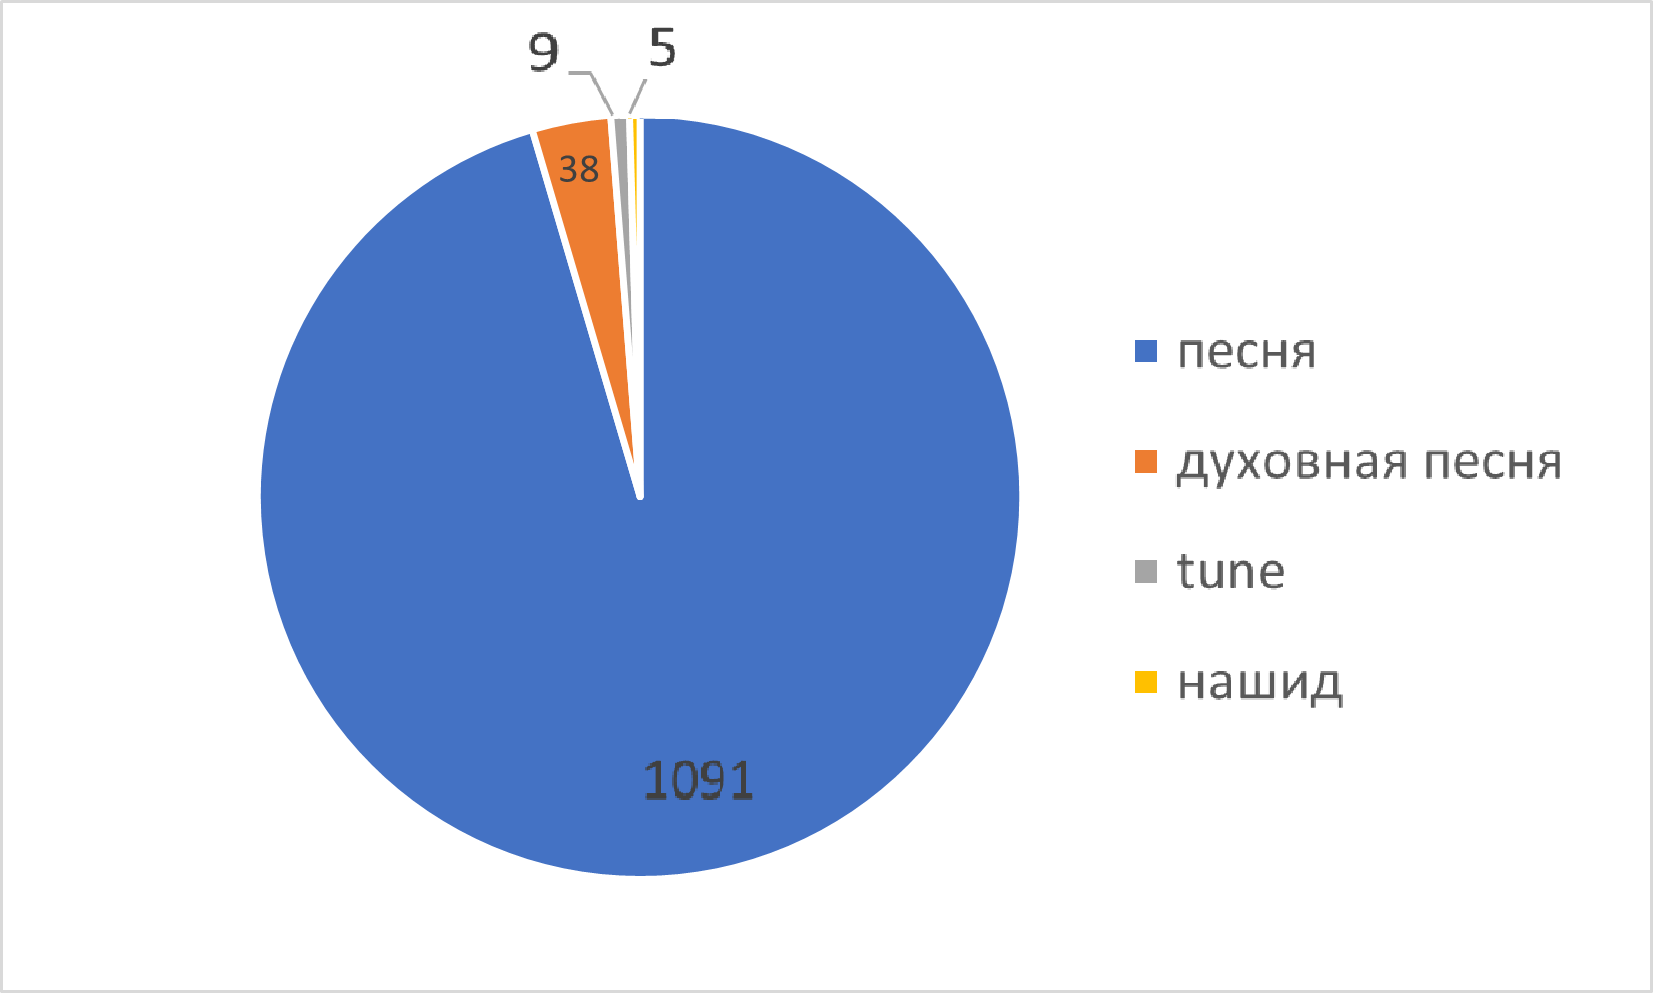
\includegraphics[width=1\textwidth]{./chapter/musical_composition/Genre_Chart_2000-2010.png}
	\caption[Круговая диаграмма музыкальных жанров за 2000--2010 годы во всем мире]{Круговая диаграмма музыкальных жанров за 2000--2010 годы во всем мире. Ссылка на SPARQL-запрос: \href{https://w.wiki/6Vx6}{https://w.wiki/6Vx6}.}%
	\label{fig:Genre_Chart_2000_—_2010}%
\end{marginfigure}

Из результатов запроса~\ref{lst:count_of_pieces_of_music_in_each_subclass} и запроса~\ref{lst:count_of_pieces_of_music_in_each_subclass_2}, можем сделать вывод, что жанры музыкальных произведений первого пика, не отличаются от жанров второго. На второй диаграмме~\ref{fig:Genre_Chart_2000_—_2010}, видим, что 95,5\,\% музыкальных произведений написаны в жанре <<песня>>. В жанре <<духовная песня>> количество музыкальных произведений по сравнению с рис.~\ref{fig:Genre_Chart_1960_—_1980} уменьшилось почти в 4 раза. А такие музыкальные жанры, как: <<переведенная песня>> и <<лирико-музыкальное произведение>> на диаграмме~\ref{fig:Genre_Chart_2000_—_2010} по сравнению с диаграммой~\ref{fig:Genre_Chart_1960_—_1980} пропали.

\section{Число композиций по десятилетиям в России}
Добавим в запрос~\ref{lst:count_of_pieces_of_music_in_each_subclass_2} страну происхождения (<<Россия>> и <<СССР>>) музыкальныз произведений, а ограничение по годам в строках 7 и 8 уберём. Получим запрос~\ref{lst:The_number_of_musical_compositions_in_Russia_for_every_10_years}, подсчитывающий сколько отечественных музыкальных произведений было написано в каждом десятилетии с середины XIX века до настоящего времени.

\begin{lstlisting}[ language=SPARQL,
                    caption={\href{https://w.wiki/88ic}{ Количество музыкальных произведений в Росии и СССР за каждые 10 лет}\protect\footnotemark},
                    label=lst:The_number_of_musical_compositions_in_Russia_for_every_10_years,
                    texcl 
                    ]
# The number of musical compositions in Russia for every 10 years
#defaultView:BarChart
SELECT (STR(?date) AS ?date_str) (COUNT(?composition) AS ?count) WHERE {
      {?composition wdt:P17 wd:Q15180}               # country = USSR
  UNION {?composition wdt:P17 wd:Q159}               # country = Russia
  UNION {?composition wdt:P495 wd:Q159}    # country of origin = Russia
  UNION {?composition wdt:P495 wd:Q15180}.  # country of origin =  USSR
  ?composition wdt:P31 wd:Q105543609;     # instance of compostion
    wdt:P86 ?composer;                    # composition has a composer
    wdt:P577 ?publication.                # composition has a publication date

  BIND(YEAR(?publication) AS ?year)
  BIND((FLOOR(?year / 10 )) * 10  AS ?date)
  FILTER (!wikibase:isSomeValue(?publication)) # field "date" must be filled
}
GROUP BY ?date
ORDER BY ?date
\end{lstlisting}%
\footnotetext{Ссылка на SPARQL-запрос: \href{https://w.wiki/88ic}{https://w.wiki/88ic}.}

\begin{marginfigure}[0\baselineskip]
	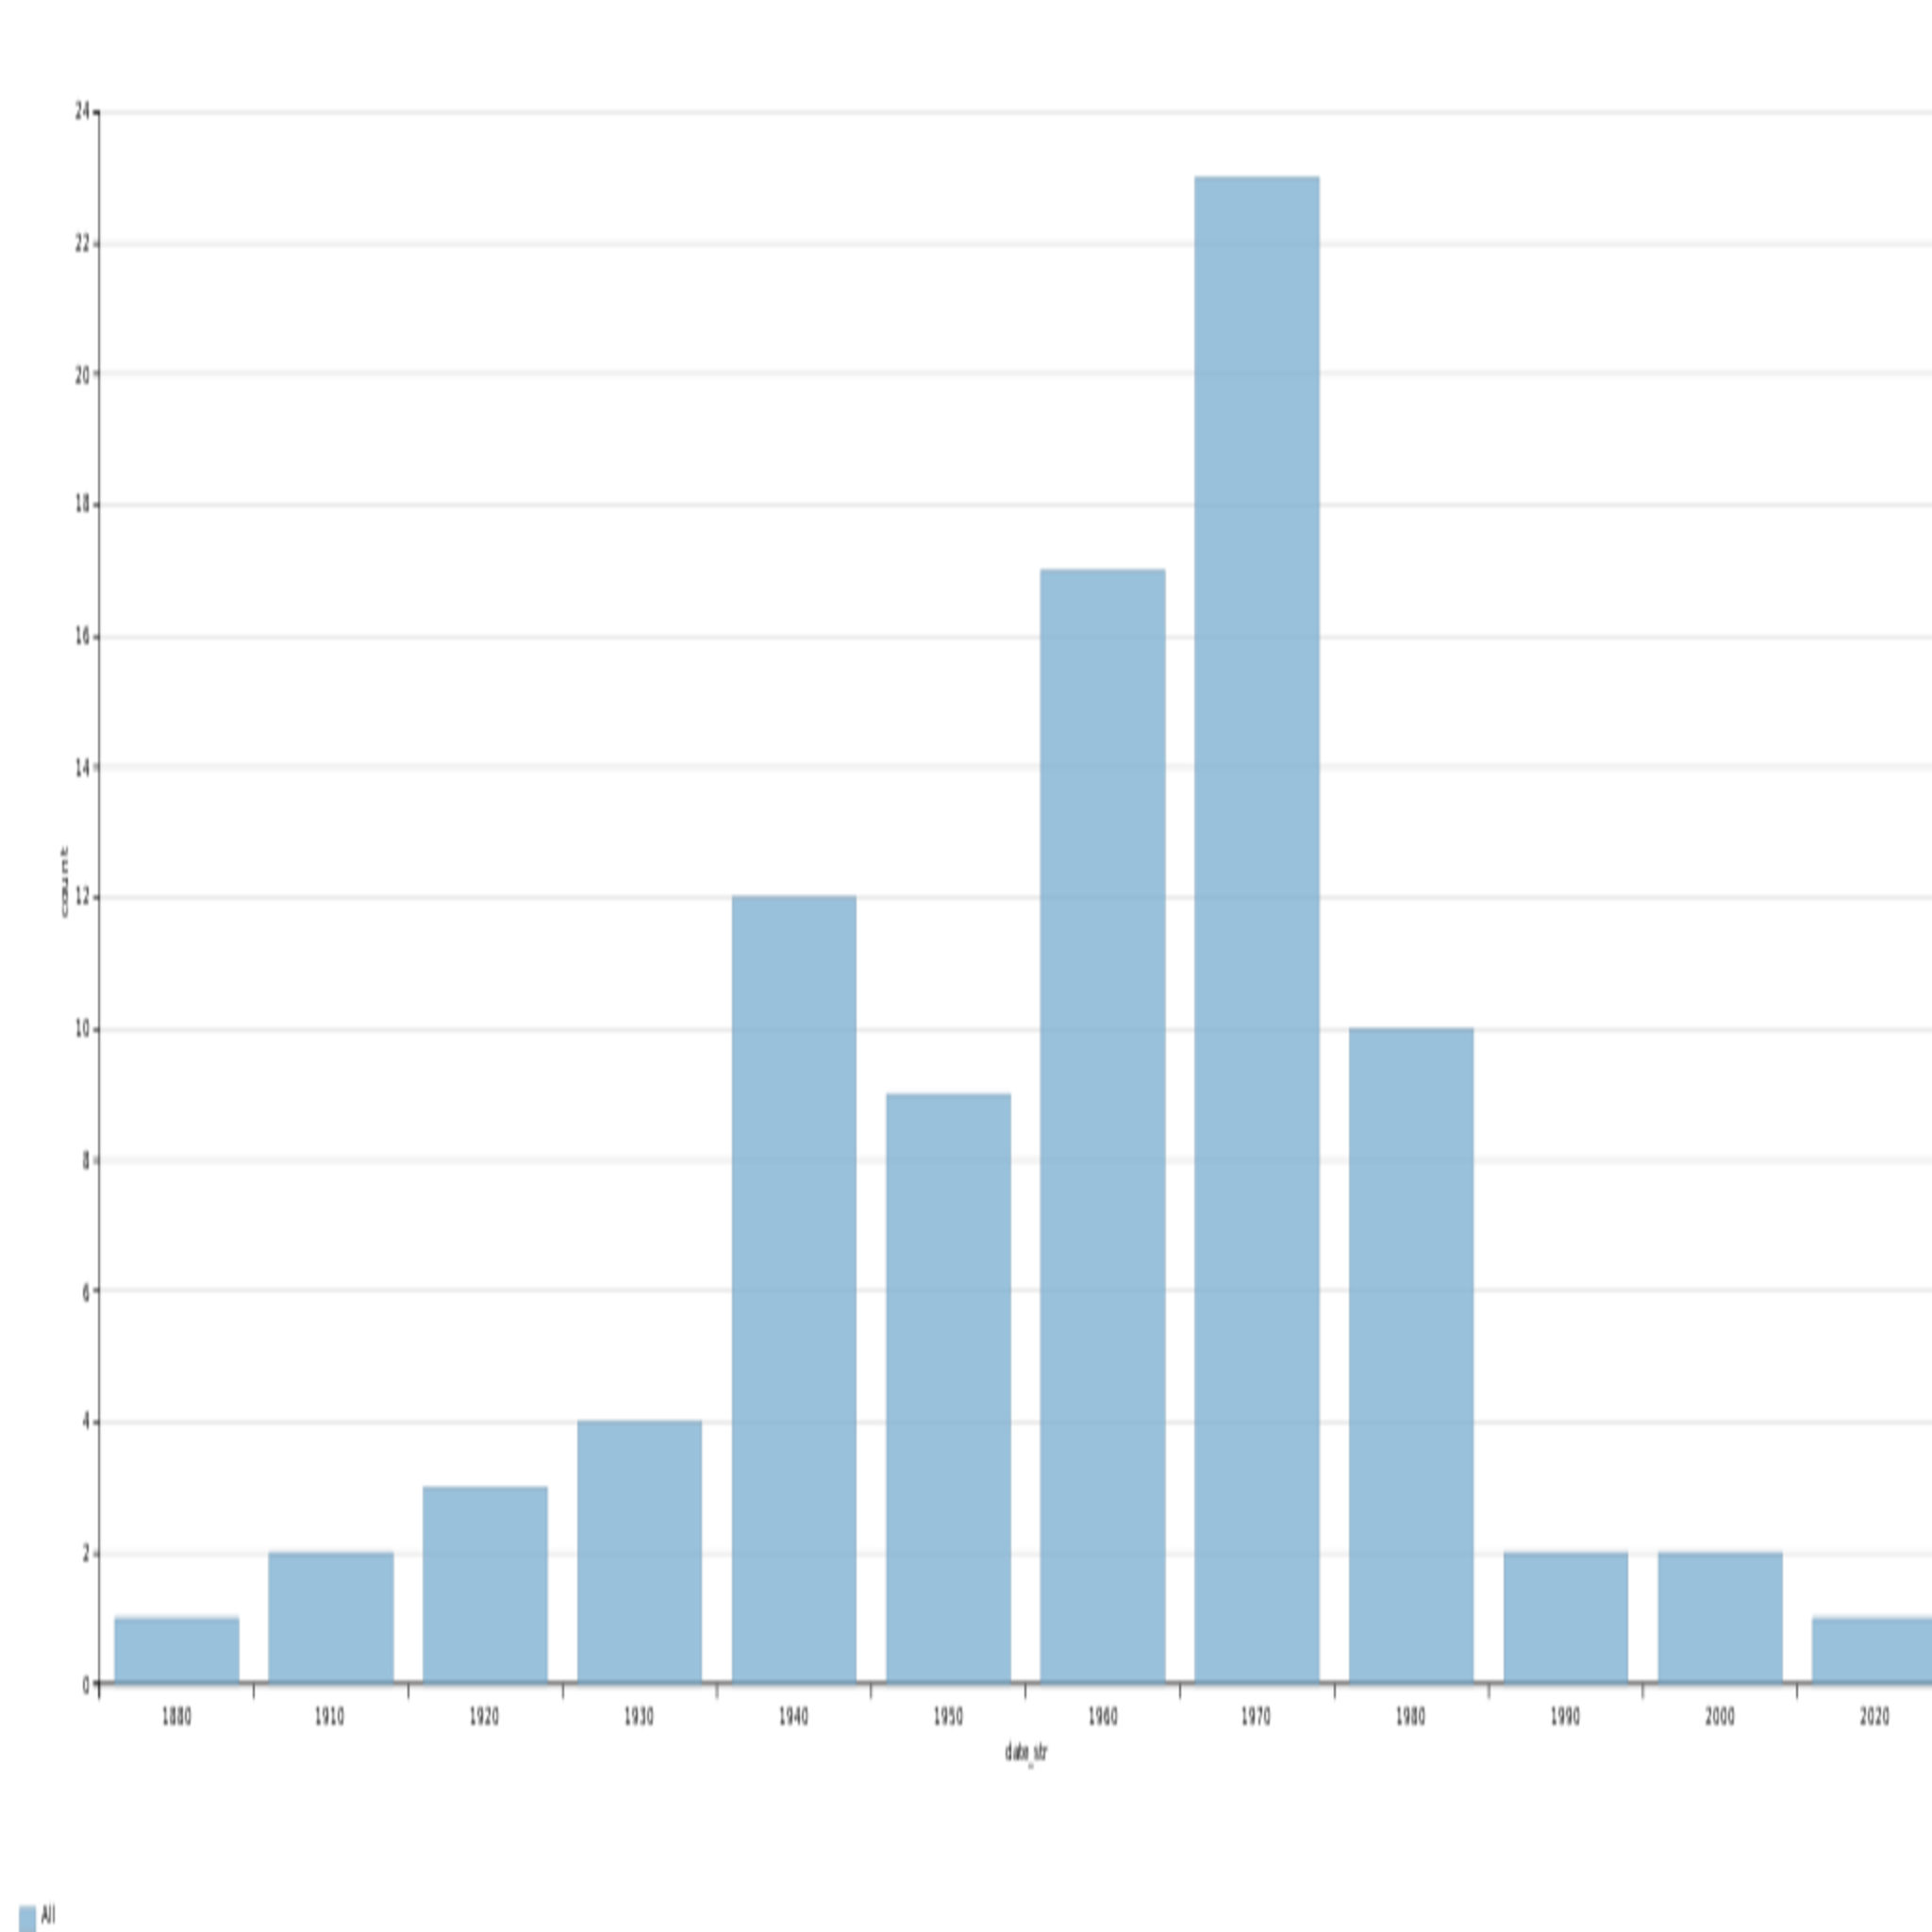
\includegraphics[width=1\textwidth]{./chapter/musical_composition/Barchart_of_The_number_of_music_compositions_in_Russia_and_USSR_every_10_years.svg.png}
	\caption[Гистограмма количества музыкальных композиций в России и СССР за каждые 10 лет с XIX века до настоящего времени]{Гистограмма количества музыкальных композиций в России и СССР за каждые 10 лет с XIX века до настоящего времени}%
\end{marginfigure}

Количество музыкальных произведений в России и СССР очень мало (97). Проанализировав несколько песен, написанных в России, таких как: <<\wdqName {Песня без слов (Кино)} {101001315}>>, <<\wdqName {Музыка нас связала} {105724079}>>, <<\wdqName {Розовое вино} {57744615}>>, не попавших в данный скрипт, стало понятно, что у этих произведений отсутствует свойство <<\wdProperty{495} {Cтрана происхождения}>>.
Далее уберём из запроса~\ref{lst:The_number_of_musical_compositions_in_Russia_for_every_10_years} строку 9 (wdt:P86 ?composer;), получим SPARQL-запрос: \href{https://w.wiki/8A8t}{https://w.wiki/8A8t}. Строка 9 ставила условие обязательного наличия композитора у музыкального произведения. Убрав эту строку, на выходе мы получаем произведения как с композиторами, так и без них. Сравним результаты обоих скриптов на диаграмме~\ref{fig:chart}. Изучив ее, можем сделать вывод, что запрос \href{https://w.wiki/8A8t}{https://w.wiki/8A8t} в основном выдаёт больше или столько же результатов, как и запрос~\ref{lst:The_number_of_musical_compositions_in_Russia_for_every_10_years}, что логично, потому что запрос \href{https://w.wiki/8A8t}{https://w.wiki/8A8t} не имеет обязательного условия наличия композитора. Но есть исключения, например: 1880-е, 1960-е. Рассмотрим, какие результаты выдают запросы за 1880 год. Запрос \href{https://w.wiki/8rd8}{https://w.wiki/8rd8} выдает 5 результатов: <<\wdqName {Всенощное бдение} {16002554}>>, <<\wdqName {String Quartet on the Theme B-la-F} {18660379}>> это произведение повторяется 4 раза. Вся проблема заключается в том, что у музыкального произведения  <<\wdqName {String Quartet on the Theme B-la-F} {18660379}>> указаны 4 композитора, поэтому оно повторяется 4 раза.


\TODO Владимир, есть два раздела (выше): (1) Количество музыкальных произведений по годам 
и (2) Число композиций по десятилетиям в России. 
У меня несколько вопросов и пожеланий, которые, надеюсь, Вы учтёте: 


\begin{marginfigure}[0\baselineskip]
	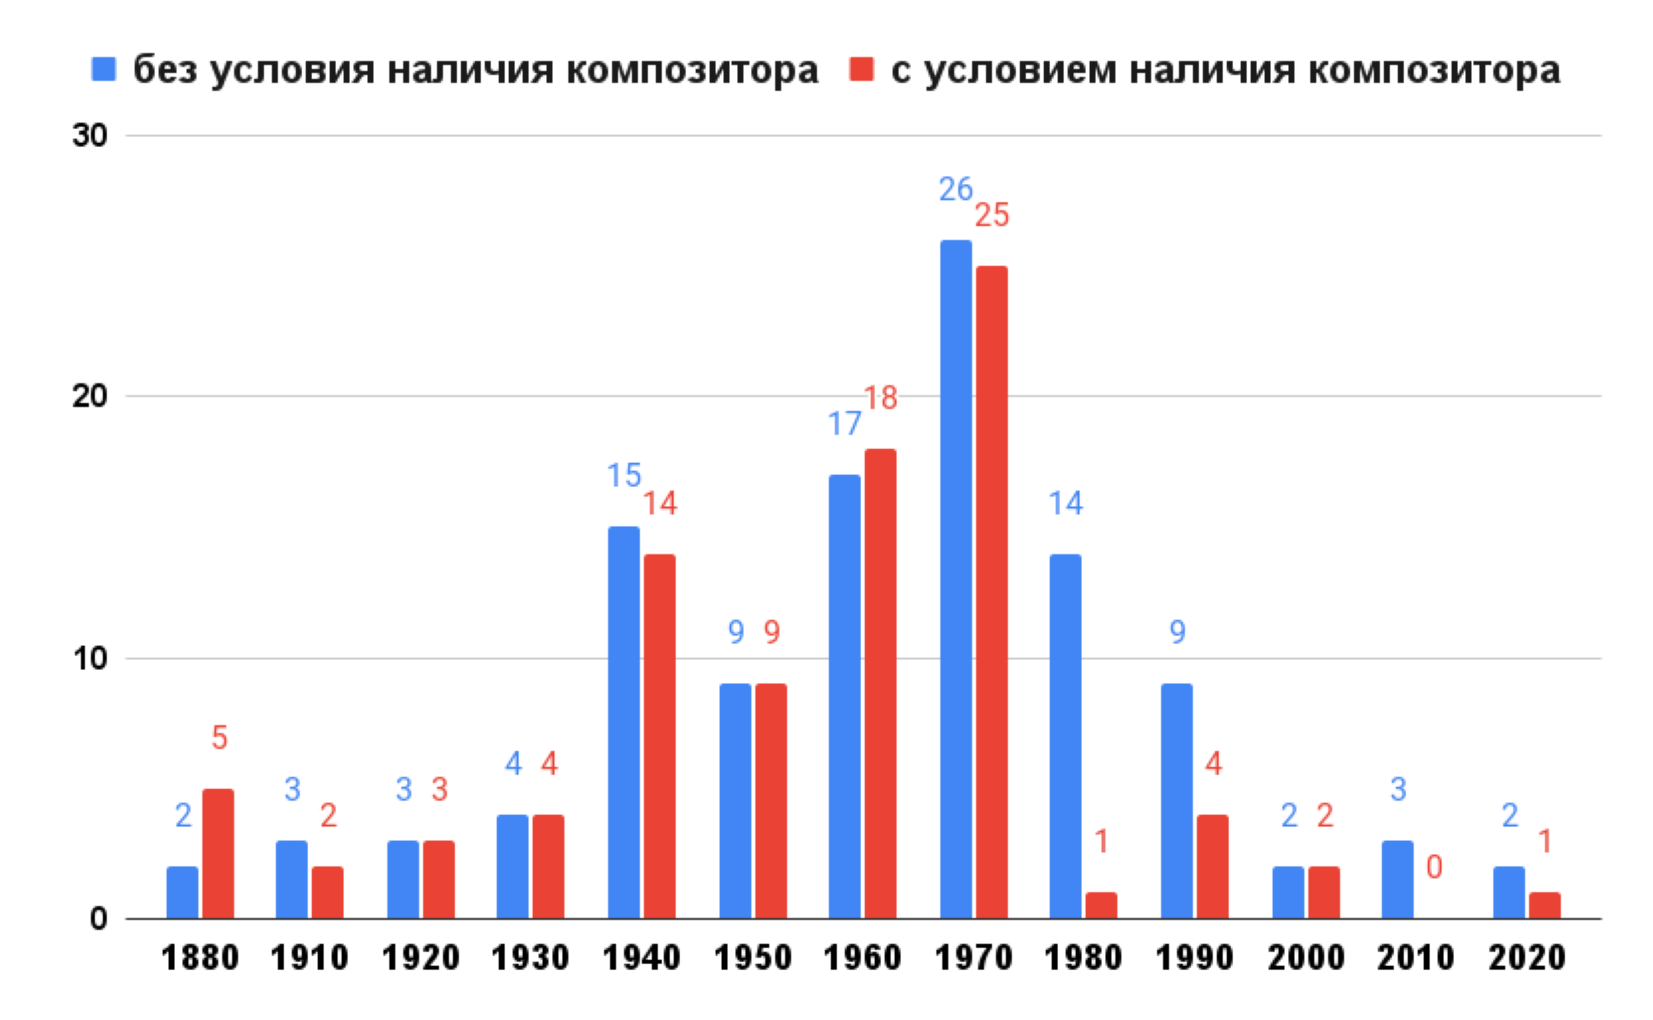
\includegraphics[width=1\textwidth]{./chapter/musical_composition/graph_of_comparison_of_readings.png}
	\caption[Диаграмма результатов запроса~\ref{lst:The_number_of_musical_compositions_in_Russia_for_every_10_years} с условием наличия композитора и без него.]{Диаграмма результатов запроса~\ref{lst:The_number_of_musical_compositions_in_Russia_for_every_10_years} с условием наличия композитора и без него.}%
	\label{fig:chart}%
\end{marginfigure}

\section{Поиск музыкальных лакун в общественном достоянии}
Задача состоит в том, чтобы найти такие музыкальные произведения, авторы которых умерли более 70 лет назад, и аудиозапись которых отсутствует на Викискладе. Найдем и упорядочим такие произведения от самых старых к новым с помощью запроса~\ref{lst:music_gaps_in_public_domain}. Существует практическая выгода и польза от~такого запроса~\ref{lst:music_gaps_in_public_domain}, поскольку видно, какие произведения можно и нужно оцифровывать (с пластинок, кассет) и загружать на Викисклад для илюстрации статей Википедии.

\begin{lstlisting}[ language=SPARQL,
                    caption={\href{https://w.wiki/88jR}{ Отсутствующие аудиозаписи музыкальных произведений, авторы которых умерли более 70 лет назад }\protect\footnotemark},
                    label=lst:music_gaps_in_public_domain,
                    texcl,
	         numbers=none
                    ]
# Search music gaps in public domain
SELECT ?composition ?compositionLabel ?publication
WHERE {
  ?composition wdt:P31 wd:Q105543609.	# instance of compostion
  ?composition wdt:P86 ?composer.		# composition has a composer
  ?composition wdt:P577 ?publication.		# composition has a publication date
  ?composer wdt:P570 ?death.			# composer has a date of death
  MINUS {?composition wdt:P51 []}.		# compositions without audio 
  FILTER(?death < "1953-01-01T00:00:00Z"^^xsd:dateTime)        # composers that passed away more than 70 years ago
  FILTER(?publication < "1953-01-01T00:00:00Z"^^xsd:dateTime)  # compositions that were published more than 70 years ago
  SERVICE wikibase:label { bd:serviceParam wikibase:language "ru,en". }
}
ORDER BY ASC(?publication)
\end{lstlisting}%
\footnotetext{Получено: \num{3771} запись на 2017 год и \num{4273} записи на 2023 год. Ссылка на SPARQL-запрос: \href{https://w.wiki/88jR}{https://w.wiki/88jR}.}

В России общественное достояние включает природные ресурсы, культурные объекты, научные достижения и образовательные ресурсы, предназначенные для общего пользования и подлежащие сохранению в соответствии с законодательством. В общем случае произведение переходит в общественное достояние в России, если с года смерти его автора прошло 70 лет. Кроме того, существует <<правило 70+4>>, согласно которому лица, трудившиеся или участвовавшие в Великой Отечественной войне, могут рассчитывать на приоритет в использовании общественных ресурсов.
\footnotetext{Ссылка на статью: \href{https://ru.wikipedia.org/?curid=31363}{https://ru.wikipedia.org/wiki/Общественное\_достояние\#Общественное\_достояние\_в\_России}.}

\section{Полнота Викиданных}
Проанализируем полноту Викиданных. Сравним количесво уникальных композиторов, предоставленных в Викиданных, с числом композиторов по другим источникам. Так же проверим, как изменяется полнота Викиданных со временем, сравнив результаты запроса~\ref{lst:BubbleChart} за~2017 год, рис.~\ref{fig:Composers2017} и за~2022 год, рис.~\ref{fig:Composers2023}.

По данным \href{https://ru.wikipedia.org/wiki/Музыкальный_словарь_Гроува}{<<Музыкального словаря Гроува>>} за всю историю человечества существовало \num{20374} композиторов.

\footnotetext{\href{https://ru.wikipedia.org/wiki/Музыкальный_словарь_Гроува}{<<Музыкального словаря Гроува>>}.}

По данным категории \href{https://ru.wikipedia.org/wiki/Категория:Композиторы_по_алфавиту}{<<Композиторы по алфавиту>>} Русской Википедии существует \num{6130} композиторов.

\footnotetext{\href{https://ru.wikipedia.org/wiki/Категория:Композиторы_по_алфавиту}{<<Композиторы по алфавиту>>}.}

По данным категории \href{https://en.wikipedia.org/wiki/List_of_composers_by_name}{<<List of composers by name>>} Английской Википедии существует \num{4685} композиторов.

\footnotetext{\href{https://en.wikipedia.org/wiki/List_of_composers_by_name}{<<List of composers by name>>}.}

Количество музыкальных композиций с заполненным свойством <<\wdProperty{86}{композитор}>> равно \num{3862}, что показывает нам запрос \href{https://w.wiki/56Rc}{https://w.wiki/56Rc}, и это с учётом того, что один композитор мог написать несколько музыкальных произведений. Например, \href{https://ru.wikipedia.org/wiki/Моцарт,_Вольфганг_Амадей}{Вольфганг Амадей Моцарт} написал \num{95} произведений, что существенно снижает количество уникальных композиторов. Полученное число \num{3862}, из результатов запроса \href{https://w.wiki/56Rc}{https://w.wiki/56Rc}, меньше, чем количество композиторов из Русской и Английской Википедии и существенно меньше, чем количество композиторов из \href{https://ru.wikipedia.org/wiki/Музыкальный_словарь_Гроува}{<<Музыкального словаря Гроува>>}, что говорит нам о неполноте Викиданных.

\begin{marginfigure}[1\baselineskip]
  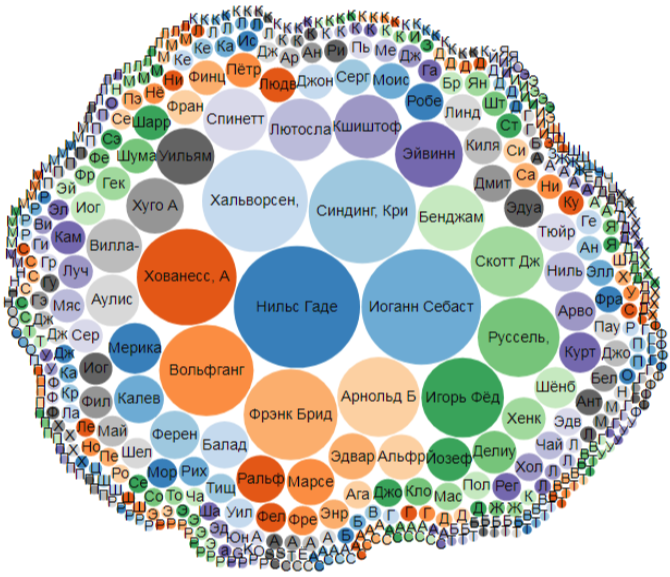
\includegraphics[width=\textwidth]{./chapter/musical_composition/Composer_all_2017.png}
  \vspace{-7pt}
  \caption[Пузырьковая диаграмма композиторов по количеству написанных композиций на~2017 год]{Пузырьковая диаграмма композиторов по количеству написанных композиций на~2017 год}%
  \label{fig:Composers2017}%
\end{marginfigure}

Запрос \href{https://w.wiki/56Rj}{https://w.wiki/56Rj} по композициям с заполненным свойством <<\wdProperty{86}{композитор}>> и свойством <<\wdProperty{495}{страна происхождения}>>, имеющим значения <<\wdqName{Российская империя}{34266}>>, <<\wdqName{СССР}{15180}>> или <<\wdqName{Россия}{159}>>, выдал всего лишь \num{8} произведений, что говорит о~невозможности анализа русских музыкальных произведений в связи с недостатком данных.

Построим  две пузырьковые диаграммы композиторов с музыкальными произведениями за 2017 год, рис.~\ref{fig:Composers2017} и за~2023 год, рис.~\ref{fig:Composers2023}.

\footnotetext{Получено: \num{773} записи. Ссылка на SPARQL-запрос: \href{https://w.wiki/85oS}{https://w.wiki/85oS}.}
\begin{lstlisting}[ language=SPARQL, numbers=none,
                    caption={\href{https://w.wiki/85oS}{ Пузырьковая диаграмма композиторов с музыкальными произведениями}\protect\footnotemark},
                    label=lst:BubbleChart,
                    texcl,
	         numbers=none
                    ]
# composers with musical compositions
#defaultView:BubbleChart
SELECT ?composer ?composerLabel (COUNT(*) AS ?count) WHERE {
  ?composition wdt:P31 wd:Q105543609; # this composition
               wdt:P86 ?composer.     # was written by the composer
  SERVICE wikibase:label { bd:serviceParam wikibase:language "ru, en" }
}
GROUP BY ?composer ?composerLabel
ORDER BY DESC(?count) ?composerLabel
\end{lstlisting}%


Запрос~\ref{lst:BubbleChart} выдает пузырьковую диаграмму изображенную на рис.~\ref{fig:Composers2017} и рис.~\ref{fig:Composers2023}.

Размер круга означает количество написанных музыкальных композиций. Диаграмма показывает, что у одних композиторов значительно больше композиций чем у других. В~первую пятерку входят \href{https://ru.wikipedia.org/wiki/Гаде,_Нильс}{Нильс Гаде} (\num{173} композиции), \href{https://ru.wikipedia.org/wiki/Бах,_Иоганн_Себастьян}{Иоганн Себастьян Бах} (\num{155} композиций), \href{https://ru.wikipedia.org/wiki/Синдинг,_Кристиан_Август}{Кристиан Август Синдинг} (\num{125} композиций), \href{https://ru.wikipedia.org/wiki/Хальворсен,_Юхан}{Юхан Хальворсен} (\num{121} композиция), \href{https://ru.wikipedia.org/wiki/Хованесс,_Алан}{Алан Хованесс} (\num{108} композиций).

%
%
\begin{marginfigure}
  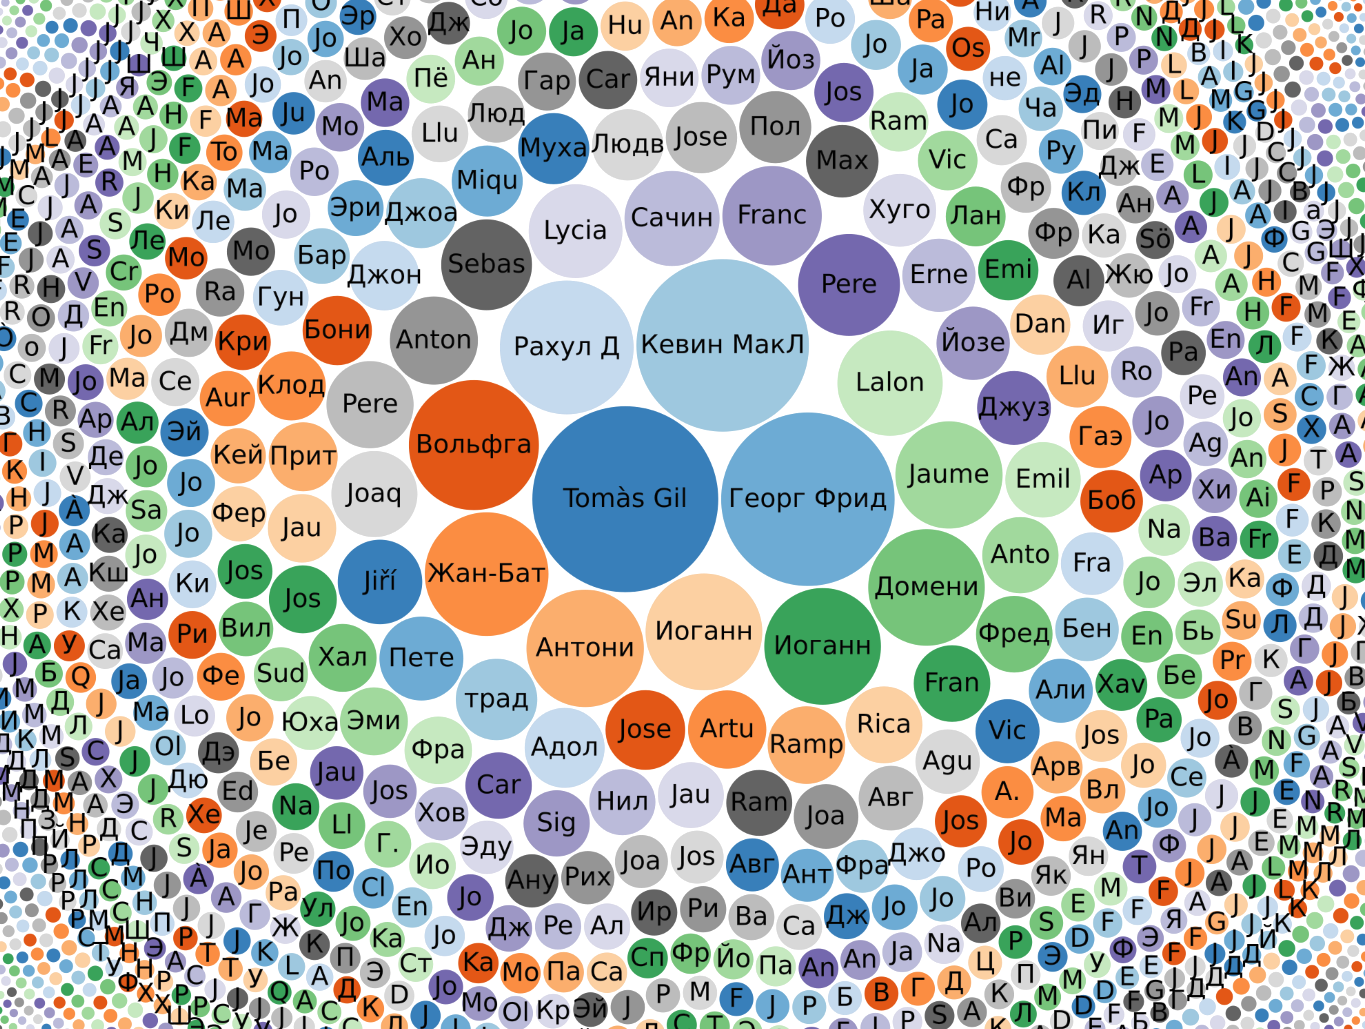
\includegraphics[width=\textwidth]{./chapter/musical_composition/Composer_all_2023_box.png}
  \vspace{-7pt}
  \caption[Пузырьковая диаграмма композиторов по количеству написанных композиций на~2023 год]
    {Фрагмент диаграммы композиторов по количеству написанных произведений на~2023 год}%
  \label{fig:Composers2023}%
\end{marginfigure}

Диаграмма~\ref{fig:Composers2023} за 2023 год позывает, как изменилось количество написанных композиций у различный композиторов. Что бы рассмотреть подробнее, добавим в конец запроса~\ref{lst:BubbleChart} строку  \lstinline|LIMIT 12|, чтобы ограничить количество записей до 12, получим следующий запрос \href{https://w.wiki/8A2h}{https://w.wiki/8A2h}, результат на рис.~\ref{fig:bubbleChart3}. Теперь сравним результаты за~2017 год и за~2023 год.
По сравнению с 2017 годом в первую пятёрку входят \href{https://ca.wikipedia.org/wiki/Tomàs_Gil_i_Membrado}{Томас Хиль Мембрадо} (\num{1437} композиций), \href{https://ru.wikipedia.org/wiki/Гендель,_Георг_Фридрих}{Гендель Георг Фридрих} (\num{1251} композиция), \href{https://ru.wikipedia.org/wiki/Маклауд,_Кевин}{Маклауд Кевин} (\num{1237} композиций), \href{https://en.wikipedia.org/wiki/R._D._Burman}{Рахул Дев Бурман} (\num{744} композиции), \href{https://ru.wikipedia.org/wiki/Моцарт,_Вольфганг_Амадей}{Вольфганг Амадей Моцарт} (\num{703} композиции). Исходя из данных диаграмм~\ref{fig:bubbleChart} и ~\ref{fig:Composers2023}, можно сделать вывод, что появились новые композиторы, которые имеют значительно больше композиций. Так же можно наблюдать имена классических композиторов, например \href{https://ru.wikipedia.org/wiki/Бах,_Иоганн_Себастьян}{Иоганн Себастьян Бах} (\num{566} композиций), тоже с существенным приростом в 411 опубликованных композиций, что говорит о дополнении Викиданных ранее неучтёнными произведениями.


\newpage
\begin{marginfigure}
  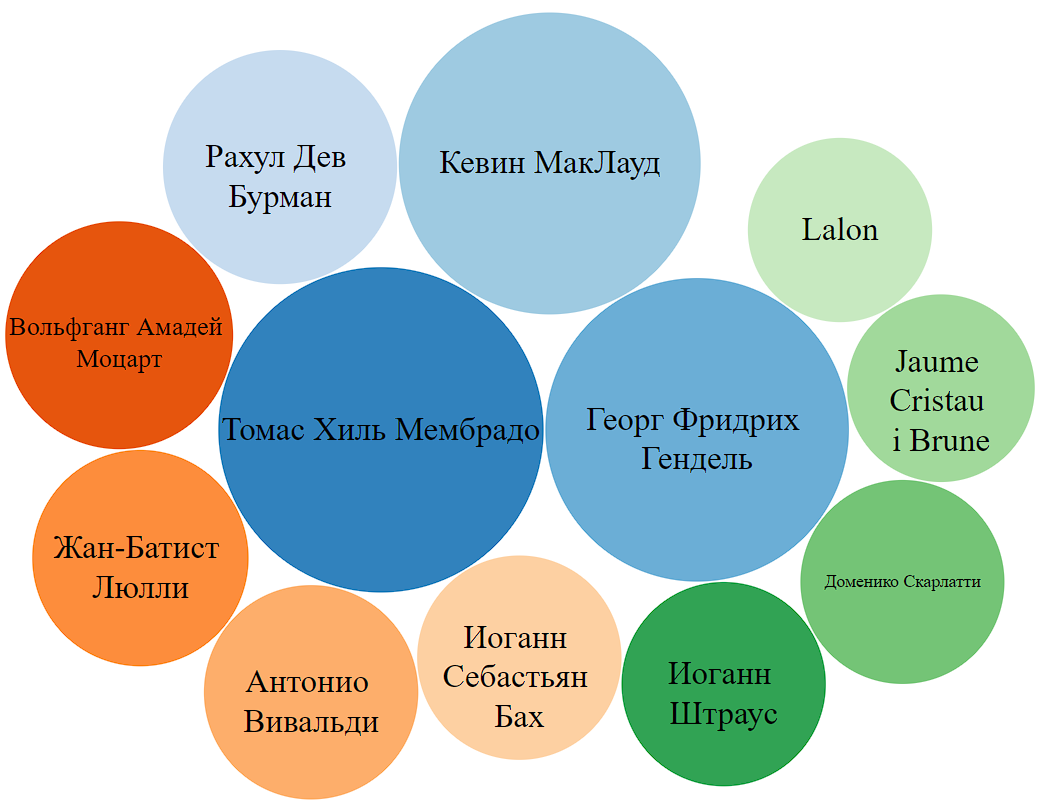
\includegraphics[width=\textwidth]{./chapter/musical_composition/Composers_12_at_2023.png}
  \caption[Диаграмма 12 композиторов с наибольшим количеством написанных музыкальных композиций на~2023 год]
          {Пузырьковая диаграмма 12 композиторов с наибольшим количеством написанных музыкальных композиций на~2023 год}%
  \label{fig:bubbleChart3}%
\end{marginfigure}


\section{Упражнения}
\begin{enumerate}
\item Найти список музыкальных композиций, созданных во время эпохи классицизма (XVII--XVIII века).
Использовать свойство: <<\wdProperty{571}{дата создания}>>.
\item Найти композитора, который написал больше симфоний, чем остальные.
Использовать свойства: <<\wdProperty{31}{экземпляр}>>, <<\wdProperty{86}{композитор}>>. Объекст: <<\wdqName {симфония} {9734}>>.
\item Построить гистограмму, на которой отображается количество музыкальных композиций группы The Beatles по году публикации.
Использовать свойства: <<\wdProperty{175}{исполнитель}>>, <<\wdProperty{577}{дата публикации}>>.

Получим следующий запрос.

\begin{lstlisting}[ 
    language=SPARQL, 
    numbers=none,
    caption={\href{https://w.wiki/9Luc}{Количество композиций группы The Beatles по годам издания}\protect\footnotemark},
    label=lst:TheBeatles,
    texcl,
]
#number of musical compositions by The Beatles by year of publication
#defaultView:BarChart
SELECT  (STR(?date) AS ?date_str) (COUNT(?composition) AS ?count)  
WHERE {
  ?composition wdt:P31 wd:Q105543609; # instance of musical work
   wdt:P175 ?executor;        # composition has a executor
  wdt:P577 ?publication.      # composition has a publication date
  FILTER (?executor = wd:Q1299).  # executor = The Beatles
  BIND(YEAR(?publication) AS ?year)
  BIND(FLOOR(?year)AS ?date)
  FILTER(?publication > "1959-01-01T00:00:00Z"^^xsd:dateTime)
  FILTER(?publication < "1971-01-01T00:00:00Z"^^xsd:dateTime) 
  FILTER (!wikibase:isSomeValue(?publication)) # field "date" must be filled
}
GROUP BY ?date
\end{lstlisting}%
\footnotetext{Получено: \num{773} записи. Ссылка на SPARQL-запрос: \href{https://w.wiki/9Luc}{https://w.wiki/9Luc}.}
Запрос~\ref{lst:TheBeatles} выдает пузырьковую диаграмму изображенную на рис.~\ref{fig:ThebeatlesBubbleChart}.

В запросе~\ref{lst:TheBeatles} мы используем свойство <<\wdProperty{175}{исполнитель}>>, вместо привычного <<\wdProperty{86}{композитор}>>. Это связано с тем, что свойство <<\wdProperty{86}{композитор}>> выдает композиторов написавших музыкальное произведение, в нашем случае нужно найти музыкальные произведения исполненные группой The Beatles.

\begin{marginfigure}
	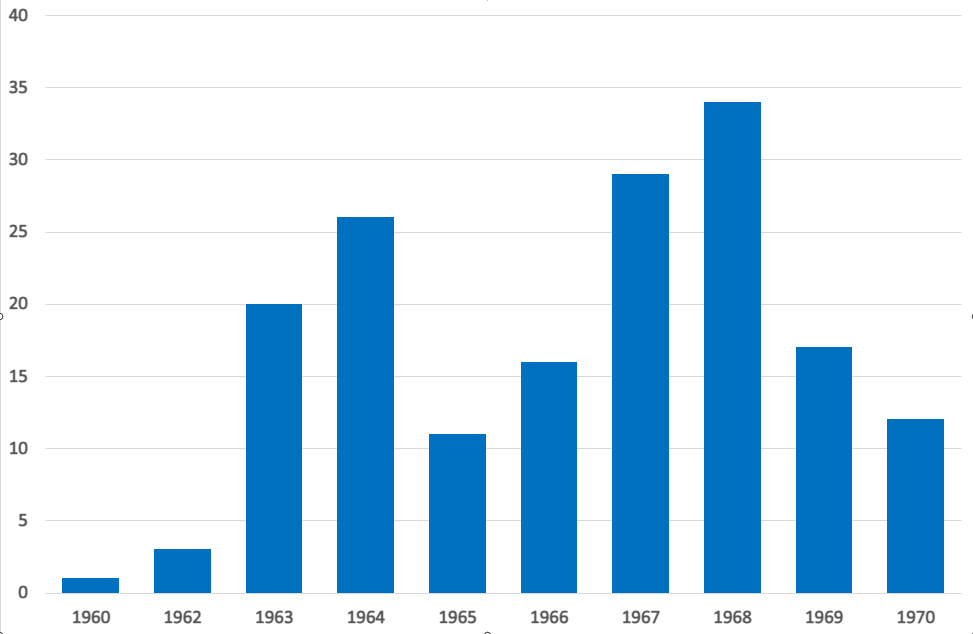
\includegraphics[width=\textwidth]{./chapter/musical_composition/BarChart_of_The_number_of_musical_comp_by The Beatles by year of publication .png}
	\caption[Гистограмма количества музыкальных композиций The Beatles по годам издания]{Ежегодное количество музыкальных композиций, выпускаемых группой The Beatles}%
 	\label{fig:ThebeatlesBubbleChart}%
\end{marginfigure}
\end{enumerate}
